\section{Additional Theory}
\label{sec:additional-theory}

\subsection{Why Maximum--Absolute and Min--Max Scaling are Unsuitable for Normally Distributed Data}

In \Cref{thm:maxabs-gev}, we show that the scaling factor in the max--abs method converges in distribution to a Gumbel distribution.

\begin{theorem}
  \label{thm:maxabs-gev}
  Let \(X_1, X_2, \dots, X_n\) be a sample of normally distributed random variables, each with mean \(\mu\) and standard deviation \(\sigma\). Then
  \[
    \lim_{n \rightarrow \infty}\Pr\left(\max_{i \in [n]} |X_i| \leq x\right) = G(x),
  \]
  where \(G\) is the cumulative distribution function of a Gumbel distribution with
  parameters
  \[
    b_n = F_Y^{-1}(1 - 1/n)\quad \text{and} \quad a_n = \frac{1}{n f_Y(\mu_n)},
  \]
  where \(f_Y\) and \(F_Y^{-1}\) are the probability distribution function and quantile function, respectively, of a folded normal distribution with mean \(\mu\) and standard deviation \(\sigma\).
\end{theorem}

The gist of \Cref{thm:maxabs-gev} is that the limiting distribution of \(\max_{i \in [n]}|X_i|\) has expected value \(b_n + \gamma a_n\), where \(\gamma\) is the Euler-Mascheroni constant. This indicates that the scaling factor strongly dependent on the sample size. In \Cref{fig:maxabs-gev}, we observe empirically that the limiting distribution agrees well with the empirical distribution in expected value even for small values of \(n\).

In \Cref{fig:maxabs-n} we show the effect of increasing the number of observations, \(n\), in a two-feature lasso model with max-abs normalization applied to both features. The coefficient corresponding to the Normally distributed feature shrinks as the number of observation \(n\) increases. Since the expected value of the Gumbel distribution diverges with \(n\), this means that there's always a large enough \(n\) to force the coefficient in a lasso problem to zero with high probability.

\begin{figure}[htpb]
  \centering
  \subcaptionbox{Theoretical versus empirical distribution of the maximum absolute value of normally distributed random variables.\label{fig:maxabs-gev}}{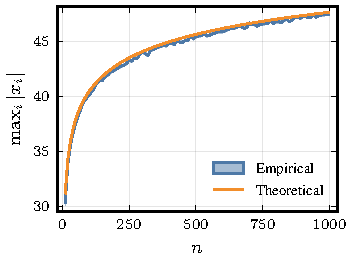
\includegraphics[]{plots/maxabs_gev.pdf}}%
  \hspace{1cm}
  \subcaptionbox{Estimation of mixed features under maximum absolute value scaling\label{fig:maxabs-n}}{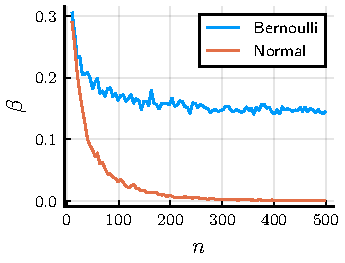
\includegraphics[]{plots/maxabs_n.pdf}}
  \caption{%
    Effects of maximum absolute value scaling.
  }
\end{figure}

For min--max scaling, the situation is similar and we omit the details here.
The main point is that the scaling factor is strongly dependent on the sample size, which makes it unsuitable for normally distributed data in several situations, such as on-line learning (where sample size changes over time) or model validation with uneven data splits.
